\documentclass{beamer}
\mode<presentation>
\usepackage{amsmath}
\usepackage{amssymb}
\usepackage{adjustbox}
\usepackage{subcaption}
\usepackage{enumitem}
\usepackage{multicol}
\usepackage{mathtools}
\usepackage{listings}
\usepackage{url}
\def\UrlBreaks{\do\/\do-}
\usetheme{Boadilla}
\usecolortheme{lily}
\setbeamertemplate{footline}
{
  \leavevmode%
  \hbox{%
  \begin{beamercolorbox}[wd=\paperwidth,ht=2.25ex,dp=1ex,right]{author in head/foot}%
    \insertframenumber{} / \inserttotalframenumber\hspace*{2ex} 
  \end{beamercolorbox}}%
  \vskip0pt%
}
\setbeamertemplate{navigation symbols}{}

\providecommand{\nCr}[2]{\,^{#1}C_{#2}} % nCr
\providecommand{\nPr}[2]{\,^{#1}P_{#2}} % nPr
\providecommand{\mbf}{\mathbf}
\providecommand{\pr}[1]{\ensuremath{\Pr\left(#1\right)}}
\providecommand{\qfunc}[1]{\ensuremath{Q\left(#1\right)}}
\providecommand{\sbrak}[1]{\ensuremath{{}\left[#1\right]}}
\providecommand{\lsbrak}[1]{\ensuremath{{}\left[#1\right.}}
\providecommand{\rsbrak}[1]{\ensuremath{{}\left.#1\right]}}
\providecommand{\brak}[1]{\ensuremath{\left(#1\right)}}
\providecommand{\lbrak}[1]{\ensuremath{\left(#1\right.}}
\providecommand{\rbrak}[1]{\ensuremath{\left.#1\right)}}
\providecommand{\cbrak}[1]{\ensuremath{\left\{#1\right\}}}
\providecommand{\lcbrak}[1]{\ensuremath{\left\{#1\right.}}
\providecommand{\rcbrak}[1]{\ensuremath{\left.#1\right\}}}
\theoremstyle{remark}
\newtheorem{rem}{Remark}
\newcommand{\sgn}{\mathop{\mathrm{sgn}}}
\providecommand{\abs}[1]{\left\vert#1\right\vert}
\providecommand{\res}[1]{\Res\displaylimits_{#1}}
\providecommand{\norm}[1]{\left\lVert#1\right\rVert}
\providecommand{\mtx}[1]{\mathbf{#1}}
\providecommand{\mean}[1]{E\left[ #1 \right]}
\providecommand{\fourier}{\overset{\mathcal{F}}{ \rightleftharpoons}}
\providecommand{\system}{\overset{\mathcal{H}}{ \longleftrightarrow}}
\providecommand{\dec}[2]{\ensuremath{\overset{#1}{\underset{#2}{\gtrless}}}}
\newcommand{\myvec}[1]{\ensuremath{\begin{pmatrix}#1\end{pmatrix}}}
\let\vec\mathbf

\lstset{
frame=single, 
breaklines=true,
columns=fullflexible
}

\numberwithin{equation}{section}

\title{MATGEO PRESENTATION}
\author{DWARAK A\\EE24BTECH11019}
\date{\today} 

\begin{document}

\begin{frame}
\titlepage
\end{frame}

\section*{Outline}
\begin{frame}
\tableofcontents
\end{frame}

\section{Problem Statement}
\begin{frame}
\frametitle{Problem Statement}
Find a relation between $x$ and $y$ such that the point $(x, y)$ is equidistant from the points $(3, 6)$ and $(-3, 4)$.
\end{frame}

\section{Solution}
\subsection{Variables Used}
\begin{frame}
    \frametitle{Variables Used}
    \begin{table}[H]    
  \centering
  \begin{tabular}[12pt]{ |c|c|c|}
    \hline
	\textbf{Variable} & \textbf{Description} & \textbf{Value} \\ 
    \hline
    $\angle B$ & Angle at vertex $\vec{B}$ & $45\degree$ \\
    \hline 
    $\angle C$ & Angle at vertex $\vec{C}$ & $120\degree$ \\
    \hline
    $K=a+b+c$ & Perimeter of $\triangle\vec{ABC}$ & $10.4cm$ \\
    \hline
\end{tabular}

\end{table}
\end{frame}

\subsection{Equidistant Point Condition}
\begin{frame}
\frametitle{Equidistant Point Condition}

If $\vec{X}$ is equidistant from points $\vec{A}$ and $\vec{B}$
\begin{align}
	\norm{\vec{A} - \vec{X}} &= \norm{\vec{B} - \vec{X}} \\
	\norm{\vec{A} - \vec{X}}^2 &= \norm{\vec{B} - \vec{X}}^2
\end{align}
Expanding the squared norms:
\begin{align}
	\norm{\vec{A}}^2 - 2\vec{A}^\top \vec{X} + \norm{\vec{X}}^2 &= \norm{\vec{B}}^2 - 2\vec{B}^\top \vec{X} + \norm{\vec{X}}^2 \\
\end{align}
\end{frame}

\subsection{Perpendicular Bisector Equation}
\begin{frame}
\frametitle{Perpendicular Bisector Equation}

The equation simplifies to
\begin{align}
        \label{eq:mat_eqn}
	\brak{\vec{A} - \vec{B}}^\top \vec{X} &= \frac{\norm{\vec{A}}^2 - \norm{\vec{B}}^2}{2}
\end{align}

Substituting the $\vec{A}$ and $\vec{B}$ values, \eqref{eq:mat_eqn} can be derived as follows

\begin{align}
    \myvec{6 \\ 2}^\top \vec{X} &= \frac{\norm{\myvec{3 \\ 6}}^2-\norm{\myvec{-3 \\ 4}}^2}{2} \\
    \myvec{6 \\ 2}^\top \vec{X} &= 10 \\
    \label{eq:line_eqn} \implies \myvec{3 \\ 1}^\top \vec{X} &= 5
\end{align}
\end{frame}

\subsection{Final Equation}
\begin{frame}
\frametitle{Final Line Equation}
Thus, from \eqref{eq:line_eqn} the line equation representing points equidistant from $\vec{A}(3, 6)$ and $\vec{B}(-3, 4)$ is:
\begin{align}
	3x + y = 5
\end{align}
The code below verifies \eqref{eq:line_eqn}
\end{frame}

\definecolor{codegreen}{rgb}{0,0.6,0}
\definecolor{codegray}{rgb}{0.5,0.5,0.5}
\definecolor{codepurple}{rgb}{0.58,0,0.82}
\definecolor{backcolour}{rgb}{0.95,0.95,0.92}


\lstset{
    language=C,
    basicstyle=\footnotesize\ttfamily,
    backgroundcolor=\color{backcolour},
    commentstyle=\color{codegreen},
    keywordstyle=\color{blue},
    numberstyle=\tiny\color{codegray},
    stringstyle=\color{codepurple},
    breakatwhitespace=false,
    breaklines=true,
    captionpos=b,
    keepspaces=true,
    numbers=left,
    numbersep=5pt,
    showspaces=false,
    showstringspaces=false,
    showtabs=false,
    tabsize=2
}
\section{C Code}
\begin{frame}[fragile,allowframebreaks]
\frametitle{C Code}
\lstinputlisting[label=mycode1]{codes/points.c}
\end{frame}

\definecolor{codegreen}{rgb}{0,0.6,0}
\definecolor{codegray}{rgb}{0.5,0.5,0.5}
\definecolor{codepurple}{rgb}{0.58,0,0.82}
\definecolor{backcolour}{rgb}{0.95,0.95,0.92}

\section{Python Code}
\lstset{
    language=Python,
    basicstyle=\ttfamily\small,
    keywordstyle=\color{blue},
    stringstyle=\color{codepurple},
    commentstyle=\color{codegreen},
    backgroundcolor=\color{backcolour},
    breaklines=true,
    breakatwhitespace=true,
    tabsize=4
}

\begin{frame}[fragile,allowframebreaks]
\frametitle{Python Code}
\lstinputlisting[label=mycode1]{codes/plot.py}
\end{frame}

\section{Plot}
\begin{frame}
\frametitle{Plot}
\begin{figure}[H]
    \centering
	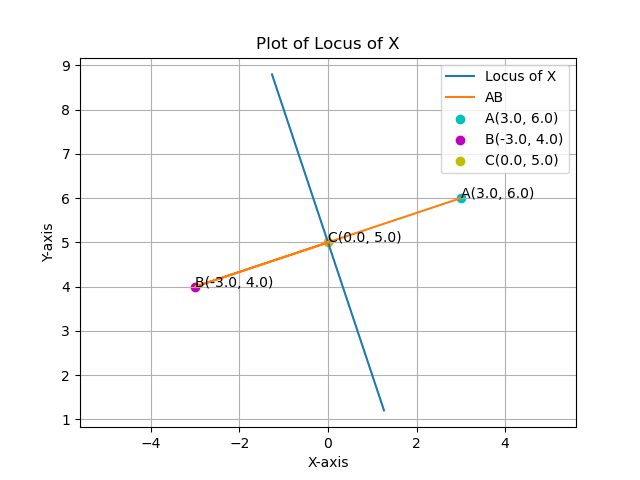
\includegraphics[width=0.8\textwidth]{figs/plot.png}
    \caption{Locus of point X, equidistant from $\vec{A}$ and $\vec{B}$}
    \end{figure}
\end{frame}

\end{document}
